\chapter{Method}
\label{sec:method}

In this chapter, the complete framework will be described. Section \ref{sec:parser} will introduce a parser that constructs valid rhythmic structures. Section \ref{sec:rejection} will describe the probabilistic elements of the parser. These are elaborated in section \ref{sec:prior} and \ref{sec:likelihood} where respectively the rhythm and expression model are discussed. Section \ref{sec:corpus} will introduce the jazz corpus. Section \ref{sec:training} will describe how the rhythm and expression model are trained on the corpus. Finally, section \ref{sec:implementation} will describe a few implementation details of the parser.

\section{Parsing Rhythms}
\label{sec:parser}

We assume that we can represent the performance $P$, of a rhythm as series of note onset times. 
\begin{equation}
\label{eq:performance}
P = [\mathrm{On}_0, \mathrm{On}_1, \cdots, \mathrm{On}_n]
\end{equation}
A rhythmic structure $R$ is a hierarchical representation of rhythm, corresponding to subdivision trees described in the previous chapter.

The approach presented here generates the most likely rhythmic structure $R$ underlying a performance $P$. During this process the parser considers all possible hypotheses of sub spans of $P$ and retains the most likely hypotheses, while rejecting the unlikely ones. We think this is computationally feasible because we assume that over a few notes, only a small number of hypotheses are worth considering. In this section we will first describe how structurally sound rhythmic analyses are generated. After that, we will outline a Bayesian model that defines how we determine whether a hypothesis is likely.

The parser we use is a slightly modified stochastic CKY chart parser \citep{Younger1967recognition}. The full algorithm and modifications are given in appendix \ref{app:parser}. A small context-free grammar augmented with some constraints will be used to generate subdivision trees. The grammar below constructs subdivision trees from onsets ($\bullet$) and ties ($*$).
\begin{align}
R &\rightarrow R\: R\\ \notag
R &\rightarrow R\: R\: R\\ \notag
R &\rightarrow \bullet\\ \notag
R &\rightarrow * \notag
\end{align}
We will restrict ourselves to duple and triple subdivisions for this study..

The CKY parser only accepts grammars that are given in the so-called Chomsky normal form (CNF). That is, all rules should be of the form $A \rightarrow B, C$ or $A \rightarrow \alpha$, where $A$, $B$ and $C$ are non-terminal symbols and $\alpha$ is a terminal symbol. Converting the grammar above to CNF results in the following grammar:
\begin{align}
\label{eq:grammar_cnf}
R &\rightarrow R\: R\\ \notag
R &\rightarrow R\: R'\\ \notag
R' &\rightarrow R\: R\\ \notag
R &\rightarrow \bullet\\ \notag
R &\rightarrow * \notag
\end{align}

Two constraints are needed to prevent the parser from generating invalid rhythmical structures. These constraints are: (1) Any set of two or three metrical durations are not allowed to combine if the first one expands directly to an onset and the others do not recursively expand to an onset. (2) Metrical durations are not allowed to combine if none of them recursively contains an onset.

\begin{figure}
\centering
\subfloat[]{
\label{fig:constraints:a}
\parbox{0.2\textwidth}{
\Tree
[ .{$\frac{1}{1}$} [ .$\bullet$ ] [ .{$\frac{1}{2}$} [ .$\bullet$ ] [ .$*$ ] ] ]
}
=
\parbox{0.2\textwidth}{
\Tree
[ .{$\frac{1}{1}$} [ .$\bullet$ ] [ .$\bullet$ ] ]
}
}
\qquad
\subfloat[]{
\label{fig:constraints:b}
\parbox{0.2\textwidth}{
\Tree
[ .{$\frac{1}{1}$} [ .{$\frac{1}{2}$} [ .$*$ ] [ .$*$ ] ] [ .$\bullet$ ] ] 
}
=
\parbox{0.2\textwidth}{
\Tree
[ .{$\frac{1}{1}$} [ .$*$ ] [ .$\bullet$ ] ] 
}
}
\caption{Redundant tree structures}
\label{fig:constraints}
\end{figure}

The first constraint prevents the parser from generating structures with an onset on the downbeat and a tie on the upbeat. An upbeat tied to a downbeat is redundant: If we tie an upbeat quarter note to a downbeat quarter note we get a half note and not two tied quarter notes. The second constraint prevents the parser from combining subdivision trees that do not contain onsets. Figure \ref{fig:constraints:a} illustrates the first constraint and figure \ref{fig:constraints:b} illustrates the second.

% Explanation of the chart parser?

This completely defines the parser. At this point however, the parser simply generates all possible interpretations of an onset list of a certain length. The next sections will describe how a probabilistic model is used to reject unlikely interpretations and retain the likely ones.

\section{Hypothesis Generation and Rejection}
\label{sec:rejection}

Subdivision trees generated by the parser can be seen as hypotheses about the rhythmic structure (some sub-span of) the performance. We will assume that the likelihood of an hypotheses given a set of performed onsets is determined by two factors: One is how well the analysis matches the observed onset times and another is likely the rhythm itself is. In other words, we want to find the \textit{posterior} probability $P(A|N)$, where $A$ is a rhythm, and $N$ is a list of note onsets. We can formulate this as a generative model where
\begin{equation}
\label{eq:model}
P(R|P) \propto P(P|R)P(R).
\end{equation}

The posterior probability $P(R|P)$ of a rhythm $R$ given a performance $P$ is proportional to $P(P|R)$, the probability that $R$ generated performance $P$ times $P(R)$, the probability of $R$ itself. $P(P|R)$ is called the \textit{likelihood} of $R$ given $P$ and $P(R)$ is called the \textit{prior} probability of $R$.

Another way to refer to the prior and the likelihood is respectively as a rhythm model and an expression model. The rhythm model should reflect intuitions about rhythms, for example that long notes tend to fall on downbeats, that duple divisions are more likely than triple divisions, etcetera. The prior used in this study will be described in section \ref{sec:prior}

The expression model defines how and to what extent we expect onsets to deviate from their idealised onsets. In our system, the expression model will be based on one observation, which we shall call the \textit{expression ratio}. The expression ratio is defined as the logarithmic ratio of downbeat length and upbeat length. In metronomic performances, we expect downbeats and upbeats to be of equal length and their ratio to one. In human performances however, it will reflect the stretching of beats. At low levels, the ratio reflects local expressive timing. A positive value at the quarter note level for example indicates that downbeats are played slightly longer than upbeats (for example as a means of emphasising them). At higher levels, above the bar-level, the expression ratio reflects global changes in tempo.

% So no tempo curves are needed

Finally, the chart parser should only keep track of hypotheses that are reasonably sensible. For this purpose, two types of beams are used: First, the per-item likelihood of the hypothesis (see section \ref{sec:training}) should be higher than a certain threshold parameter. Second, after a cell has been filled with hypotheses by the parser (see appendix \ref{app:parser} for more details), the hypotheses are ranked by their posterior probability and only the top-$n$ hypotheses are kept.

Both the rhythm and the expression model will be trained on the corpus of annotated jazz performances that was constructed for this study and which will be described in detail in section \ref{sec:corpus}.

\section{The Rhythm model}
\label{sec:prior}

The prior probability of an analysis $R$ should be an indication of how likely $R$ is a priori. Should we only use a hypothesis likelihood to assess the quality of our hypotheses, the parser would produce overly complicated analyses that try to fit the performance as close as possible. By using an rhythm model in parallel with an expression model, the parser will balance how well the analysis `fits' the performance and how likely the hypothesised rhythmic structure is by itself.

Our rhythm model will be a probabilistic context-free grammar (PCFG). A PCFG is a context-free grammar extended with probabilities for every rewrite rule. The probability of a syntax tree, produced by a PCFG can be derived by taking the product of every rule that was applied to construct the tree. In linguistics, PCFGs do not always assign probabilities to rules expanding to terminal symbols (words) since there are too many of them. In our case however, there are only two terminal symbols so we can assign probabilities to rules expanding to onsets or ties as well.

Note that there is only one non-terminal symbol in our grammar, namely $R$, so the probability of a rule expansion is given by
\begin{equation}
P(R \rightarrow S) = P(S) = \frac{\mathrm{count}(S)}{N},
\end{equation}
where S is a string of symbols and N is the total number of $R$ symbols in the training set. 

The probability of a subdivision tree $R$ can be described as 
\begin{equation}
P(R) = \prod_{R' \rightarrow S \in R} P(R' \rightarrow S).
\end{equation}
where $R' \rightarrow S \in R$ refers to every rule expansion of some symbol $R$ to a string of symbols $S$ that is recursively contained in $R$.


\section{The Expression model}
\label{sec:likelihood}


\subsection{Hypothesis representation}
\label{sec:hypothesis_representation}

\begin{figure}
\Tree
[ .{$\frac{1}{1}$} [ .{$\frac{1}{2}$} [ .$\bullet$ ] [ .$\bullet$ ] ] [ .$*$ ] ]
\caption{A rhythmic analysis, which can be represented as the nested list $((\bullet, \bullet), *)$.}
\label{fig:smalltree}
\end{figure}

A subdivision tree represents a rhythmic structure, but it does not keep track of the onsets associated with the structure. In order to be able to say anything about the likelihood of an analysis, we need to have information about the onsets it contains. Therefore we will introduce a distinction between a rhythmic analysis $R$, produced by the grammar in (\ref{eq:grammar_cnf}) and a \textit{hypothesis} $h$. 

A subdivision tree is essentially a syntax tree, which, as any syntax tree, can be represented as a nested list. The tree in figure \ref{fig:smalltree} for example, can also be written as $((\bullet, \bullet), *)$. Hypotheses have a similar structure but also keep track of onsets on on the down- and upbeats. The 3-tuple below completely specifies a hypothesis.
\begin{align}
h = (H, B, O)\\ \notag
H = [h_0, \cdots, h_d]\\ \notag
B = [b_0, \cdots, b_d]\\ \notag
O = [o_0, \cdots, o_d] \notag
\end{align}
where $d$ is the division of $h$, $H$ is a list of nested hypotheses and $B$ is a list of predicted down- and upbeats that will be constructed using the \textsc{combine} function introduced later in this section. $O$ is a list of actual onsets and may contain $*$ symbols when no onsets are present at some positions. Both $B$ and $O$ only contain onsets on the level of the hypothesis, that is, they contain the down- and upbeat(s) of the hypothesis and their length is always the same as the amount of units the hypothesis divides in. The predicted downbeat of an hypothesis is $B_0$. The predicted upbeats of an hypothesis are $B_i$ where $i > 0$. When a hypothesis governs only a single onset, both $B$ and $O$ may contain $*$ symbols.

At this point it may be useful to point out that we can theoretically specify $B$ and $O$ to be functions of $h$ as their contents can be derived directly from a hypothesis. The hypothesis representation would then be identical to the rhythmic structure representation $R$ except for containing actual onset times at the leaf nodes instead of $\bullet$ symbols. However, given the complexity of the \textsc{combine} function we have chosen to represent the $B$ and $O$ lists explicitly on each node in the subdivision tree.

A single onset is represented as a hypothesis with zero nested hypotheses: \[(\emptyset, [\textrm{On}_i], [\textrm{On}_i]),\] where $\textrm{On}_i$ is an absolute onset time at position $i$ in some performance $P$. Similarly, a single tie is represented as: \[(\emptyset, [*], [*]).\] Combining these hypotheses yields \[([(\emptyset, [*], *), (\emptyset, [\textrm{On}_i], \textrm{On}_i)], [*, On_i], [*, On_i]).\] See for example figure \ref{fig:complexonsets:a}. Both the list of predicted beats $B$ and the list of onsets $O$ contain the $*$ symbol here. When this hypothesis combines with other onsets, the \textsc{combine} function will fill in the estimated onsets of $*$ in the list of beats $B$, but not in the list of onsets $O$. When the \textsc{observations} function is introduced in section \ref{sec:observations} it will become clear why the list of onsets $O$ is needed.

Estimating the likelihood of a hypothesis is done in a two-step process. The first step is a bottom-up process where the down- and upbeats of every hypothesis is estimated. This process will be described in section \ref{sec:combination}. The second step is a top down process that generates, given some hypothesis, an observation vector containing feature vector/expression ratio pairs. This process is described in section \ref{sec:observations}. The likelihood of these observations given their feature vectors can be determined after the expression model is trained on a corpus. The training procedure is described in section \ref{sec:training}.

For every observation an expression ratio, a feature vector $\varphi$ will be generated. We have already observed in section \ref{sec:rejection} that the expression ratio reflects different concepts as different levels, therefore one feature we will be using is the \texttt{level} at which the expression ratio was observed. We will use another feature reflecting the \texttt{division} of the metrical unit in which the expression ratio was observed. The resulting feature vector is:
\begin{equation}
\label{eq:features}
\varphi = [\texttt{level}, \texttt{division}].
\end{equation}
\texttt{level} is defined bottom-up, so level one is the deepest level of the tree.


\subsection{Combination}
\label{sec:combination}

A hypothesis is said to \textit{govern} a set of onsets if the hypothesis recursively contains these onsets. The \textsc{combine} function cannot estimate down- and upbeats when of a hypothesis that only governs a single onset. Such hypotheses are treated as a \textit{complex onset}. The hypothesis in figure \ref{fig:complexonsets:a} for example is treated as an onset at relative position $0.5$, the hypothesis in figure \ref{fig:complexonsets:b} is treated as an onset with relative position $0.75$.

\begin{figure}
\centering
\subfloat[complex onset: $0.5$]{
\label{fig:complexonsets:a}
\parbox{4cm}{\centering
\Tree
[ .{$\frac{1}{1}$} [ .$*$ ] [ .$\bullet$ ] ] 
}
}
\subfloat[complex onset: $0.75$]{
\label{fig:complexonsets:b}
\parbox{4cm}{\centering
\Tree
[ .{$\frac{1}{1}$} [ .$*$ ] [ .{$\frac{1}{2}$} [ .$*$ ] [ .$\bullet$ ] ] ] 
}
}
\caption{Complex onsets (single-onset analyses).}
\label{fig:complexonsets}
\end{figure}

The goal of the \textsc{combine} function is to get the best possible estimates of where the up and downbeats of a hypothesis are. The algorithm works roughly as follows. The input is a list $H$ containing two or three hypotheses. These will be the child nodes of the hypothesis that the combine function is building. The algorithm iterates through the list of hypotheses. If a hypothesis is an onset, the position of the onset and the absolute onset are added to \textit{onsets}. The position is a number between 0 and 2 or 0 and 3, depending on the number of hypotheses in $H$. If a hypothesis is a complex onset, its complex position, determined by the function \textsc{complexPostion}, and absolute onset are added to \textit{complexOnsets}. If a hypothesis suggests a downbeat, this downbeat and its position are added to \textit{onsets}.

\begin{algorithm}[h!]
\caption{Combine hypotheses}
\label{alg:combination}
\begin{algorithmic}
\Function{combine}{$H$}
	\State $d \leftarrow$ \Call{length}{$H$}
	\State onsets $\leftarrow \emptyset$
	\State complexOnsets $\leftarrow \emptyset$
	\For{$i \leftarrow 0,d$}
		\State $(H', B', O') \leftarrow H_i$
		\If{$H' = \emptyset$ \textbf{and} $B \neq [*]$}
			\State \textbf{append} ($i, H'_i$) \textbf{to} onsets
		\Else
			\If{$B'_0 \neq *$}
				\State \textbf{append} $(i, B'_0)$ \textbf{to} onsets
			\If{$O'_0 \neq *$}
				\State \textbf{append} $(i, O'_0)$ \textbf{to} $O$
			\EndIf
			\Else
				\State $p$, complexOnset $\leftarrow$ \Call{complexPosition}{$H'_i$}
				\State \textbf{append} ($i + p$, complexOnset) \textbf{to} complexOnsets
			\EndIf
		\EndIf
	\EndFor
	\If{\Call{length}{onsets} $\leq 1$}
		\State \textbf{append} complexOnsets \textbf{to} onsets
	\EndIf
	\State $B \leftarrow$ \Call{fill}{onsets, $d$}
	\State \textbf{return} $(H, B, O)$
\EndFunction
\end{algorithmic}
\end{algorithm}

Once the algorithm has iterated thought $H$, the algorithm checks whether there is an onset on the downbeat. If there is not, the \textsc{downbeat} function attempts to estimate the downbeat from the list of onsets. We assume that an interval based on one or more complex positions is less reliable than an interval based on intervals between downbeats. Only if \textit{onsets} contains less than two onsets, \textit{complexOnsets} is added to it. When the combined length of \textit{onsets} and \textit{complexOnsets} is 1, this hypothesis governs only one onset and the list of beats will only contain that onset and one or more ties. If the combined \textit{onsets} and \textit{complexOnsets} contains more than one onset, the \textsc{downbeat} function estimates downbeat from these onsets.

In a practical implementation, every hypothesis should also keep track of the first onset before and after the hypothesis. This can be used later to restrict endlessly adding ties to the hypothesis.

\subsection{Observing the expression ratio}
\label{sec:observations}

The combination process combines hypotheses makes sure that every hypothesis governing more than one note contains an estimated downbeat. This information is used by the \textsc{observations} function to transform a hypothesis $h$ to a list of observed expression ratios with feature vectors. As mentioned before, we define an the expression ratio to be the logarithmic ratio of the observed upbeat and downbeat length.

For any hypothesis $h = (H, B, O)$, we can calculate the expression ratio given that we know the (estimated or actual) onset of the downbeat, $h_0$ and the (estimated or actual) next downbeat. Since a hypothesis can be divided into more than two units, there may be more than one expression ratio per hypothesis. We define the \textit{relative position} of a beat to be zero for the downbeat, one for the first upbeat and two for the second upbeat. The expression ratio for a hypothesis with division $d = \textsc{division}(h)$, onsets $O = \textsc{onsets}(h)$, predicted beats $B = \textsc{beats}(h)$, next downbeat $B_d$, beat onset $O_i$ is calculated in the following fashion:
\begin{align}
\label{eq:expression}
\mbox{expression ratio} &= \log\left(\frac{(O_i - B_0) / i}{(B_d - O_i) / (d - i)}\right) & \text{for every $i$ where $i > 0$ and $O_i \neq *$.}
\end{align}

The \textsc{observations} function is used to derive downbeat and next downbeat estimates for any hypothesis that contains more than one onset and all the sub-hypotheses it recursively contains. The main intuition of this approach is that downbeat intervals provide the most reliable information about the local tempo. 

The \textsc{observations} function is a top-down recursive function. It is initialised with a hypothesis $h$, the downbeat of $h$ and the next downbeat. Since we have not yet observed the next downbeat for the top-level hypothesis $h$, we simply set it to the division of $h$ times the inter-onset interval of the downbeat and the first upbeat of $h$ (given that $h$ governs more than one onset, the combination process already provided estimates for every beat in $B$). So for a hypothesis $h = (H, B, O)$, the algorithm is initialised as follows: $\textsc{observations}(h, B_0, *, \textsc{length}(H) \times (B_1 - B_0))$.

The \textsc{observations} function is given in algorithm \ref{alg:observations}. The first step of the function is to initialise the estimated length $l$ as the onset of the next downbeat minus the onset of the downbeat. The division $d$ is initialised as the number of nested hypotheses (which is equivalent to the length of $H$, $B$ or $O$). Then, the set of feature vector/expression ratio pairs $S$ is initialised as an empty set. Finally the $*$ symbol is appended to the list of onsets.

Now the algorithm iterates through all every beat in the hypothesis (in this study there are can be no more than three beats in a hypothesis). For every beat position $i$ where $i > 0$ and $O_i \neq *$ the expression ratio is calculated as in equation \ref{eq:expression}. The requirements $i > 0$ and $O_i \neq *$ ensure that the expression ratio is only calculated for upbeats that contain actual onsets. 

For every beat position in $h$, the algorithm will calculate the downbeat and next downbeat for the nested hypothesis at that position, these values are stored in $b_{\mathrm{down}}$ and $b_{\mathrm{up}}$. 
For some beat position $i$, where $0 < i < d$, $b_{\mathrm{down}}$ is estimated by
\begin{equation}
\label{eq:beatonset}
b_{\mathrm{down}} = \mathrm{downbeat} + l * i/d.
\end{equation}
If an onset has been estimated by the combination process, which indicated by $B_i \neq *$, this onset is used instead. Since the combination process will always have estimated onsets for $h$s governing more than one onset, equation \ref{eq:beatonset} is only used when $h$ governs a single onset.

Given $b_{\mathrm{down}}$ the position of the next downbeat, $b_{\mathrm{up}}$ is estimated by:
\begin{equation}
b_{\mathrm{up}} = b_{\mathrm{down}} + l/d.
\end{equation}
This estimate should be equivalent to the onset at position $i+1$. If there is an onset at position $i+1$, this onset is preferred to the actual onset.

Finally, the recursive step of the algorithm calls \textsc{observations}($h', b_{\mathrm{down}}, b_{\mathrm{up}}$) for every nested hypothesis $h'$ of $h$. The algorithm stops and returns an empty set when $h$ contains no nested hypothesis, which means it represents an onset or tie.


\begin{algorithm}[h!]
\caption{Generate observations}
\label{alg:observations}
\begin{algorithmic}
\Function{observations}{$h$, downbeat, nextDownbeat}
	\State $H, B, O \leftarrow h$
	\State $d \leftarrow$ \Call{length}{$H$}
	\State $l \leftarrow$ nextDownbeat - downbeat
	\State $S \leftarrow \emptyset$
	\State \textbf{append} * \textbf{to} $O$
	\For {$i \leftarrow 0,d$}
		\If {$O_i \neq *$ \textbf{and} $i \neq 0$}
			\State $\varphi \leftarrow$ (\Call{depth}{$h$}, $d$)
			\State $r \leftarrow$ \Call{expression\textunderscore ratio}{downbeat, nextDownbeat, $B_i$, $i$, $d$}
			\State \textbf{append} ($\varphi$, r) \textbf{to} $S$
		\EndIf	
		\State $H', B', O' \leftarrow H_i$
		\If {$H' \neq \emptyset$}
			\State $b_{\mathrm{down}} \leftarrow \mathrm{downbeat} + l * i/d$
			\If {$B_i \neq *$}
				\State $b_{\mathrm{down}} \leftarrow B_i$
			\EndIf
			\State $b_{\mathrm{up}} \leftarrow b_{\mathrm{down}} + l/d$
			\If {$O_{i+1} \neq *$}
				\State $b_{\mathrm{up}} \leftarrow O_{i+1}$
			\EndIf
			\State \textbf{append} \Call{observations}{$(H', B', O'), b_{\mathrm{down}}, b_{\mathrm{up}}$} \textbf{to} $S$
		\EndIf
	\EndFor
	\State \textbf{return} $S$
\EndFunction
\end{algorithmic}
\end{algorithm}



%Constraints of the corpusparser (a parser that only allows metronomic performances)

%Single note analysis constraints

%Constraint in adding ties


%Introducing triple divisions introduces ambiguities between triple divisions or more complicated constructions of duple divisions (that are quite unlikely).


\section{Data Preparation}
\label{sec:corpus}

To train the parser's rhythm model and expression model, a corpus of amateur jazz performances was prepared. The corpus contains jazz and latin standards that were scraped off the the web by \citet{Wild:10}. The performances are generally of good quality and are played in a relatively constant tempo. In its original form, the corpus was a set of multi-track MIDI files containing both tracks played by a human performer and tracks generated by a computer in metronomic time.

MIDI files represent music as a list of note-on and note-off events, corresponding to key presses and key releases. Every event has the parameters pitch, velocity and delta-time. Delta-time specifies the time between this events and the last one, pitch is the pitch of the key that was pressed, velocity is the velocity with which the key was pressed or released.

%Our parser will be trained and evaluated on monophonic jazz melodies, played by a human performer. Monophonic tracks that were likely to be played by humans were filtered out automatically. This was done by assuming that tracks played by humans contained a lot of variation in onset velocity and in inter-onset intervals due to imperfect timing. From this subset of performed tracks, tracks containing melodies where selected by hand.

After the filtering process, 20 tracks were left containing unique performances of 12 different melodies. These MIDI files where converted to note lists of the following format:
\begin{align*}
N &= [n_0, n_1, \cdots, n_N],\\
n_i &= (\mathrm{On}_i, \mathrm{Pitch}_i, \mathrm{Velocity}_i),
\end{align*}
where $N$ is a note list containing notes $n_0$ to $n_N$, $\mathrm{On}_i$, $\mathrm{Pitch}_i$ and $\mathrm{Velocity}_i$ is the onset time in micro seconds, pitch and velocity of the $i^{\mathrm{th}}$ note. A very simple annotation format was chosen: a list of metrical onsets, measured in quarter notes, with pointers to the corresponding notes in $N$. There are three types of annotations: an onset, a grace note and a rest. Although this study will ignore grace notes and rests, they are included for completeness and potential future use of the corpus.

An annotation $A$, corresponding to note list $N$ has the following format:
\begin{align*}
A &= [a_0, a_1, \cdots, a_N],\\
a_j &= (\mathrm{Position}_j, \mathrm{Pointer}_j, \mathrm{Type}_j),
\end{align*}
where $\mathrm{Position}_j$ is a metrical position, measured in quarter notes, $\mathrm{Pointer}_j$ is a pointer that points to the index of the corresponding note in the note list and $\mathrm{Type}_j$ indicates whether this annotation is an onset, a grace note or a rest. Since rests are not included in the note list, their pointer is irrelevant and points to zero. 

Some extra information is added to the annotation when it is stored. The annotation $A$ is stored in a 3-tuple $(T, t, A)$, where $t$ is the tempo in beats per minute and $T$ is the time signature. The time signature contains the number of beats per measure, or measure division $d$ and the number by which we have to divide 1 to get the units of those beats $u$, where $u$ can be any positive real number (although $u$ is almost always a power of 2). 
\begin{equation*}
T = (d, u)
\end{equation*}
This representation is identical to the musical representation of time signature. The information in the time signature combined with onsets measured in quarter notes can be used to derive the measure number of every onset in the annotation. To do so, quarter notes ($q$) are first converted to beats ($b$) as follows: $b = qu/4$. A position measured in beats can then be converted to a position measured in bars ($m$) like so: $m = b/d$

Many performances in the corpus where played in swing. Although swing may refer to many intentional deviations from metronomic timing, a very common one is to play notes that are notated as eighth notes as eighth note triplets, the so-called `shuffle'. This is illustrated in figure \ref{fig:swing}. The score usually notates swung notes as in figure \ref{fig:swing:a}, whereas the notes are played as in figure \ref{fig:swing:b} and \ref{fig:swing:c}. Writing swung notes as in \ref{fig:swing:a} is just a notational convention, and often the scores contain instructions to play eighth notes as in figure \ref{fig:swing:b}.

The manual annotation process resulted in lists of metrical onset times. Combined with the time signature and tempo information, the metrical onset times can be converted to any metrical unit and to metronomic onset times. Deriving te subdivision trees from this information was done semi-automatically. A simple parser with a flat prior and a likelihood function that only allowed metronomic timing was used to generate parses for every item in the corpus. From these results correct parses where selected by hand. A subdivision tree for the swing example is shown in figure \ref{fig:swing:c}. 


\begin{figure}
\centering
\subfloat[Rhythm notation]{
\label{fig:swing:a}
\centering
\begin{tabular}{|c|}
\hline
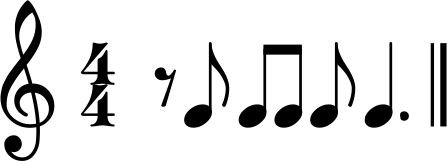
\includegraphics[scale=0.3]{img/aint_misbehavin}\\
\hline
\end{tabular}
}
\\
\subfloat[Annotation]{
\label{fig:swing:b}
\centering
\begin{tabular}{|c|}
\hline
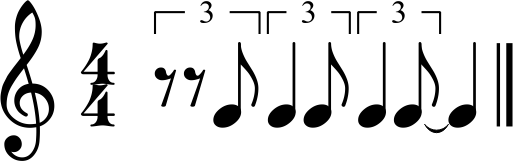
\includegraphics[scale=0.3]{img/aint_misbehavin_swung}\\
\hline
\end{tabular}
}
\\
\subfloat[Parsetree]{
\label{fig:swing:c}
\centering
\Tree 
[ .{$\frac{1}{1}$} [ .{$\frac{1}{2}$} [ .{$\frac{1}{4}$} [ .$*$ ] [ .$*$ ] [ .$\bullet$ ] ] [ .{$\frac{1}{4}$} [ .$\bullet$ ] [ .$*$ ] [ .$\bullet$ ] ] ] [ .{$\frac{1}{2}$} [ .{$\frac{1}{4}$} [ .$\bullet$ ] [ .$*$ ] [ .$\bullet$ ] ] [ .$*$ ] ] ]
}
\caption{Swung notes.}
\label{fig:swing}
\end{figure}

The result of this process for Thelonious Monk's standard Blue Monk is shown in figure \ref{tab:annotation}. A full list of jazz standards in the corpus is given in appendix \ref{app:corpus}.

\begin{figure}[h!]
\begin{tabular}{|l|}
\hline

\parbox{\linewidth}{
The performance onsets in milliseconds:
}\\

$P = [32, 348, 504, 836, 1940, 2240, 2420, 2728]$\\


\parbox{\linewidth}{
Metrical onsets in quarter notes. Triple divisions are rounded to two digits:
}\\

$ A = [0.0, 0.66, 1.0, 1.66, 4.0, 4.66, 5.0, 5.66]$\\


\parbox{\linewidth}{
Rhythmic analysis generated by a simple parser and selected by hand:
}\\

\Tree
[ .{$\frac{1}{1}$} [ .{$\frac{1}{2}$} [ .{$\frac{1}{4}$} [ .{$\frac{1}{8}$} [ .$\bullet$ ] [ .$*$ ] [ .$\bullet$ ] ] [ .{$\frac{1}{8}$} [ .$\bullet$ ] [ .$*$ ] [ .$\bullet$ ] ] ] [ .$*$ ] ] [ .{$\frac{1}{2}$} [ .{$\frac{1}{4}$} [ .{$\frac{1}{8}$} [ .$\bullet$ ] [ .$*$ ] [ .$\bullet$ ] ] [ .{$\frac{1}{8}$} [ .$\bullet$ ] [ .$*$ ] [ .$\bullet$ ] ] ] [ .$*$ ] ] ]
\\


\parbox{\linewidth}{
Score generated from the subdivision tree combined with pitch information. The bar duration was set to level 1/2 of the subdivision tree:}\\

\includegraphics[scale=0.4]{img/blue_monk}\\
\hline
\end{tabular}
\caption{A performance of the first two bars of Thelonious Monk's Blue Monk, the corresponding metrical onsets, rhythmic analysis and score generated from the analysis.}
\label{tab:annotation}
\end{figure}


\section{Training}
\label{sec:training}

The model is trained using maximum likelihood estimation. First, for all items in the train set, the observed parameters are and their corresponding feature vectors, the resulting feature vector/parameter pairs $(\phi, p)$ are stored in a set S. Second, we train two parameter vectors, $\mu$ and $\sigma$ to contain the expected expression ratio $r$ and standard deviation of $r$ for every feature vector $\phi$ like so:
\begin{align}
\label{eq:training}
\mu_\phi &= \frac{1}{|S|} \sum_{(p | (p, \phi) \in S))} p, \\ 
\sigma_\phi &= \frac{1}{|S|} \sum_{(p | (p, \phi) \in S)} (\mu - p)^2. \notag
\end{align}
Since we use a very simple feature vector, these parameters do not need to be smoothed.

Given the parameter vectors $\mu$ and $\sigma$, estimated by \ref{eq:training}, the likelihood of a set of observations $S$ containing feature/expression ratio pairs $(\varphi, r)$, observed in some hypothesis $h$ is given by:
\begin{equation}
\label{eq:h_likelihood}
\mathcal{L}(S|\mu, \sigma) \propto \prod_{(\varphi, r) \in S} \exp\left(-\frac{(\mu_\varphi - r)^2}{2\sigma_\varphi^2}\right).
\end{equation}

As mentioned in section \ref{sec:rejection}, a hypothesis is rejected if the per-item likelihood is lower than a certain threshold, the beam parameter. The per-item likelihood is defined as

\begin{equation}
\label{eq:per_obs_likelihood}
\mathcal{L}(S| \mu, \sigma) \mbox{ per item } \propto \exp\left(-\frac{1}{|S|}\sum_{(\varphi, r) \in S} \frac{(\mu_\varphi - r)^2}{2\sigma_\varphi^2}\right).
\end{equation}

The beam parameter is set by taking the minimum value of the per-item likelihood of each subdivision tree in the train set. 

\section{Implementation}
\label{sec:implementation}

To make the parser computationally tractable, a few optimisations were needed. It was already mentioned that the parser uses a beam parameter to reject unlikely hypotheses. In addition to that a few extra measures had to be taken.

First of all, the \textsc{observations} function returns no parameters for hypotheses containing a single onset (complex onsets). Their probability is always one and theoretically ties could be added endlessly. To restrict this the parser maintains a small list of allowed single note analyses. This list is compiled by taking all single-note analyses found in the labelled corpus.

Second of all, the corpus contains only 4/4 time signatures, therefore triple divisions are allowed only at note level. All allowed triple divisions are shown in figure \ref{fig:triples}. 

\begin{figure}
$\bullet$
\Tree
[ .{$\frac{1}{1}$} [ .$*$ ] [ .$\bullet$ ] ] 
\Tree
[ .{$\frac{1}{1}$} [ .$*$ ] [ .$*$ ] [ .$\bullet$ ] ] 
\Tree
[ .{$\frac{1}{1}$} [ .$*$ ] [ .{$\frac{1}{2}$} [ .$*$ ] [ .$\bullet$ ] ] ] 
\Tree
[ .{$\frac{1}{1}$} [ .$*$ ] [ .{$\frac{1}{2}$} [ .{$\frac{1}{4}$} [ .$*$ ] [ .$\bullet$ ] ] [ .$*$ ] ] ] 
\caption{Some of the allowed single-note analyses.}
\label{fig:singlenotes}
\end{figure}

\begin{figure}
\Tree
[ .{$\frac{1}{1}$} [ .$*$ ] [ .$*$ ] [ .$\bullet$ ] ] 
\Tree
[ .{$\frac{1}{1}$} [ .$\bullet$ ] [ .$*$ ] [ .$\bullet$ ] ]
\Tree 
[ .{$\frac{1}{1}$} [ .$\bullet$ ] [ .$\bullet$ ] [ .$\bullet$ ] ]
\caption{Allowed triple divisions.}
\label{fig:triples}
\end{figure}
% Beam
% Triple divisions
% Best-n
% Max depth
%
% Chart parsing, beam, prior, likelihood, 
